\documentclass[mathserif, 11pt, t]{beamer}

\input{beamer_setup.tex}

\newcommand{\bc}[1]{\textcolor{blue}{\mathbf{#1}}}

\begin{document}

\titlepage{California precipitation extremes, 1950--1999}{Mickey Warner}{AMS 263 --- Stochastic Processes}{22 March 2017}

\begin{frame}{Introduction}

Data:
\begin{itemize}[label=$\cdot$]
\item Observation product spanning 50 years
\item Daily measurements summed to produce daily total
\end{itemize}
\bigskip

Goal:
\begin{itemize}[label=$\cdot$]
\item Characterize the tail of the distribution
\item Make inferences based on extreme value theory
\end{itemize}
\end{frame}

\begin{frame}{Introduction --- Data}
\begin{center}
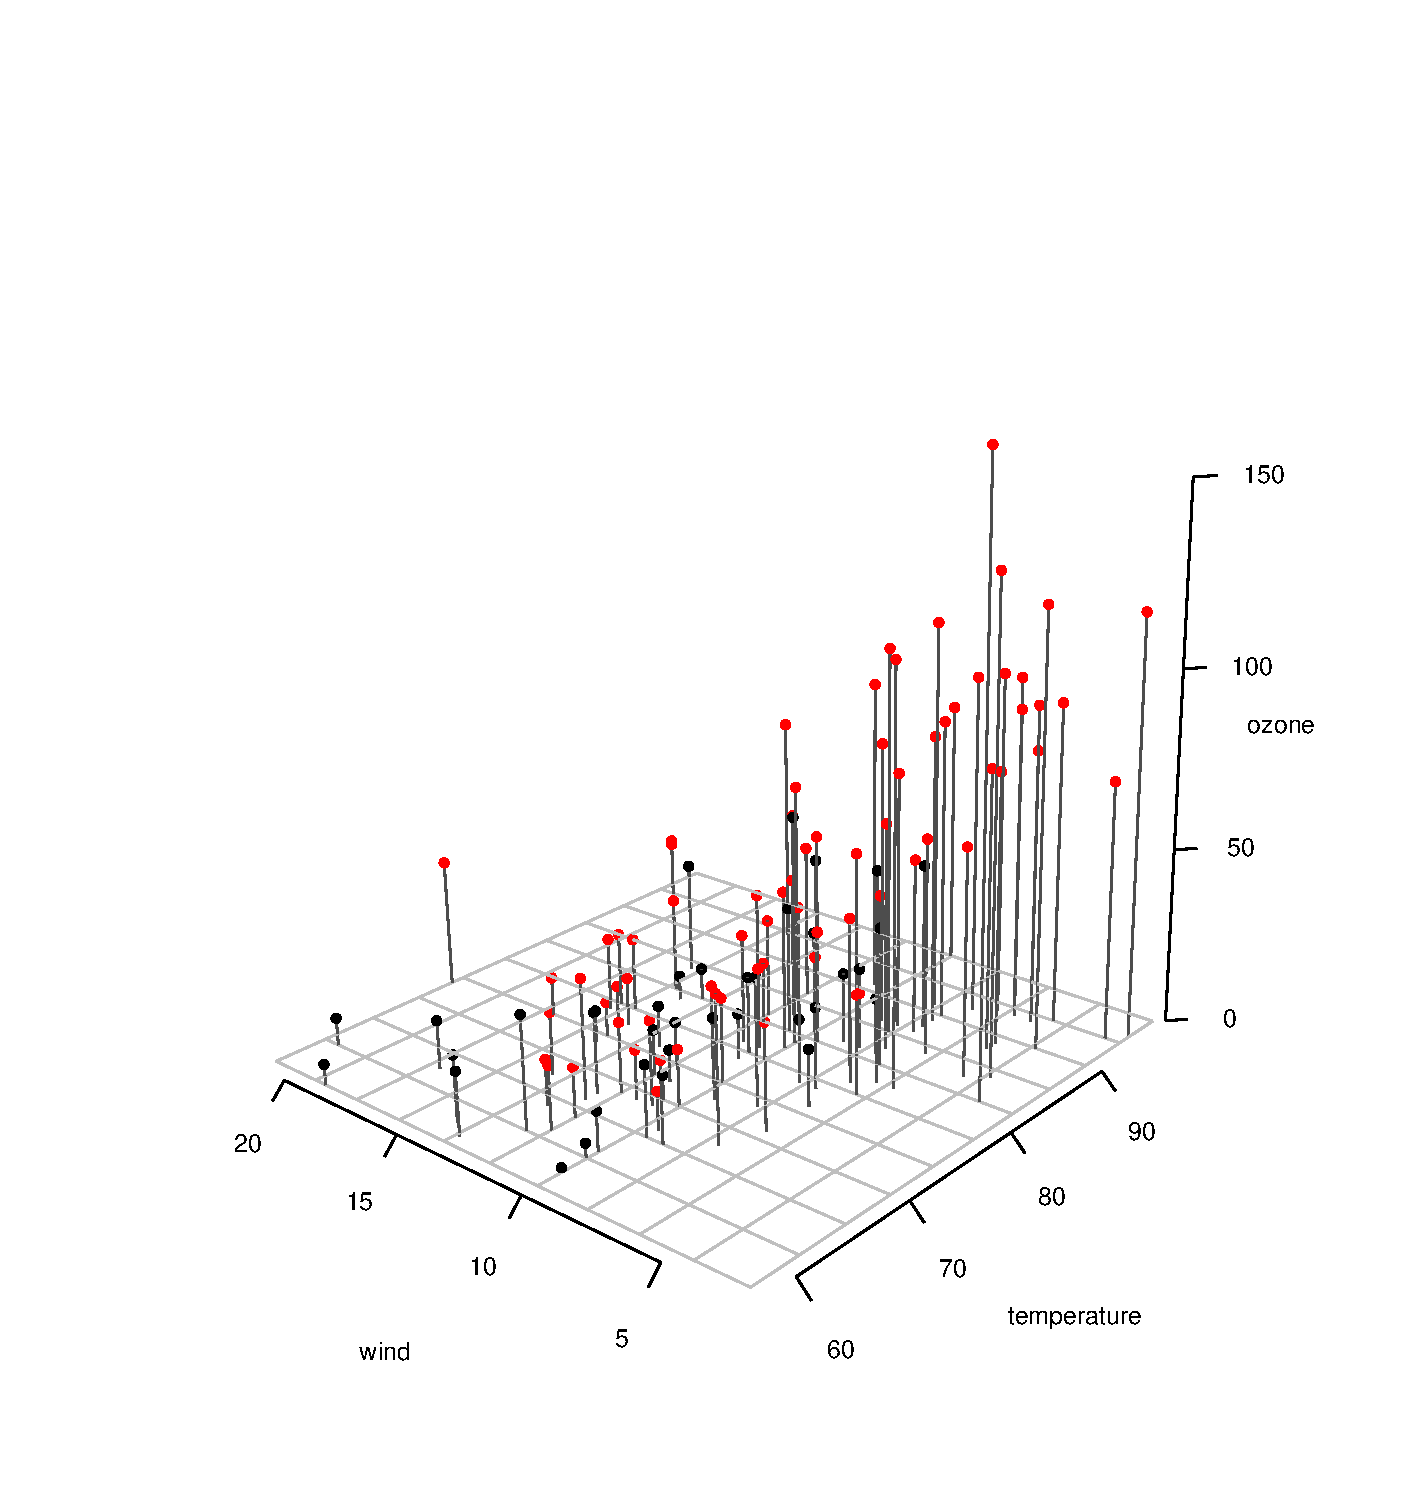
\includegraphics[scale=0.30]{../figs/data.pdf}
\end{center}
\end{frame}

\begin{frame}{Introduction --- Extremes}
\begin{center}
\includegraphics[scale=0.35]{../figs/tail.pdf}
\end{center}
\end{frame}

\begin{frame}{Poisson process characterization of extremes}

\textbf{Theorem}: Let $X_1$,$X_2$,\ldots be a series of independent and identically distributed random variables for which there are sequences of constants $\{a_n>0\}$ and $\{b_n\}$ such that
\[ \Pr\{(M_n - b_n)/a_n \leq z \} \rightarrow G(z), \]
where
\[ G(z) = \exp\left\{-\left[1+\xi\left(\frac{z-\mu}{\sigma}\right)\right]^{-1/\xi}\right\}, \]
and let $z_{-}$ and $z_{+}$ be the lower and upper end points of $G$, respectively. (Note, $M_n = \max(X_1,\ldots, X_n)$)
\end{frame}

\begin{frame}{Poisson process characterization of extremes}

\textbf{Theorem continued}: Then, the sequence of point processes
\[N_n = \{(i/(n+1),(X_i-b_n)/a_n):i=1,\ldots,n\} \]
converges on regions of the form $(0,1)\times[u,\infty)$, for any $u>z_{-}$, to a Poisson process, with intensity measure on $A=[t_1,t_2]\times[z,z_{+})$ given by
\[ \Lambda(A)=(t_2-t_1)\left[1+\xi\left(\frac{z-\mu}{\sigma}\right)\right]^{-1/\xi} \]
\qed
\end{frame}

\begin{frame}{Poisson process characterization of extremes}

\textbf{Theorem (restated)}: Let $X_1,\ldots,X_n$ be a series of independent and identically distributed random variables, and let 
\[ N_n = \{(i/(n+1),X_i):i=1,\ldots,n\}. \]
Then, for sufficiently large $u$, on regions of the form $(0,1)\times[u,\infty)$, $N_n$ is approximately a Poisson process, with intensity measure on $A=[t_1,t_2]\times(z,\infty)$ given by
\[ \Lambda(A)=(t_2-t_1)\left[1+\xi\left(\frac{z-\mu}{\sigma}\right)\right]^{-1/\xi} \]
\qed
\end{frame}

\begin{frame}{Likelihood}

Select a high threshold $u$, and set $A=(0,1)\times[u,\infty)$. Denote the $N(A)$ observations in $A$ by $\{(t_1,x_1),\ldots,(t_{N(A)},x_{N(A)})\}$.
\bigskip

The (restated) theorem leads to the following likelihood, with $[t_1,t_2]=[0,1]$:
\[ L_A(\mu,\sigma,\xi; x_1,\ldots,x_n) = \exp\{-\Lambda(A)\}\prod_{i=1}^{N(A)}\lambda(t_i,x_i) \]
\[ \propto \exp\left\{-n_y\left[1+\xi\left(\frac{u-\mu}{\sigma}\right)\right]^{-1/\xi}\right\}\prod_{i=1}^{N(A)}\sigma^{-1}\left[1+\xi\left(\frac{x_i-\mu}{\sigma}\right)\right]^{-1/\xi-1} \]

\end{frame}

\begin{frame}{Likelihood}

By convention, $n_y$ is chosen to be the number of years of observations. In our example, $n_y=50$.
\bigskip

This results in parameters $(\mu,\sigma,\xi)$ that correspond to the annual maximum distribution.
\bigskip

The threshold $u$ must be chosen to be large enough so the approximation holds, but not so large that we have too few data to work with.

\end{frame}


\begin{frame}{Time-varying parameters}

We let $\mu=\mu_t = \beta_0 + \beta_1\cos(2\pi/365\times t) + \beta_2\sin(2\pi/365\times t)$, corresponding to an annual cycle for the location parameter.
\bigskip

Similar adjustments are made for $\log \sigma$, and $\xi$.
\bigskip

This gives is model flexibility and the Poisson process handles the changes fine.

\end{frame}


\begin{frame}{Return levels}

The return level $z_m$ is the value that is exceeded on average once every $m$ years, and $z_m$ satisfies
\[ 1-\frac{1}{m} = \Pr\{\max(X_1,\ldots,X_n)\leq z_m\} \approx \prod_{i=1}^n p_i \]
where $p_i = 1 - n^{-1}[1+\xi_i(z_m-\mu_i)/\sigma_i]_{+}^{-1/xi_i}$ and $x_+=\max(0,x)$.
\bigskip

If there is no time-varying components to the parameters, then this simplifies. Otherwise, we need to solve for $z_m$ using numerical methods.
\end{frame}



\begin{frame}{Results --- time-varying threshold}
\begin{center}
\includegraphics[scale=0.30]{../figs/threshold.pdf}
\end{center}
\end{frame}

\begin{frame}{Results --- rate of exceedance}
\begin{center}
\includegraphics[scale=0.30]{../figs/exceedance_loc.pdf}
\end{center}
\end{frame}

\begin{frame}{Results --- diagnostics}
\begin{center}
\includegraphics[scale=0.30]{../figs/diag.pdf}
\end{center}
\end{frame}

\begin{frame}{Results --- posterior distributions}
\begin{center}
\includegraphics[scale=0.30]{../figs/post_mu.pdf}
\end{center}
\end{frame}

\begin{frame}{Results --- posterior distributions}
\begin{center}
\includegraphics[scale=0.30]{../figs/post_sig.pdf}
\end{center}
\end{frame}

\begin{frame}{Results --- posterior distributions}
\begin{center}
\includegraphics[scale=0.30]{../figs/post_ksi.pdf}
\end{center}
\end{frame}

\begin{frame}{Results --- 10-year return levels (by day)}
\begin{center}
\includegraphics[scale=0.30]{../figs/return10.pdf}
\end{center}
\end{frame}

\begin{frame}{Results --- 20-year return levels (by day)}
\begin{center}
\includegraphics[scale=0.30]{../figs/return20.pdf}
\end{center}
\end{frame}

\begin{frame}{Results --- 50-year return levels (by day)}
\begin{center}
\includegraphics[scale=0.30]{../figs/return50.pdf}
\end{center}
\end{frame}

\begin{frame}{Conclusion}

The distributions for the three parameters were sensitive to my choice of time-varying threshold. More work needs to be considered in selecting an appropriate threshold.
\bigskip

There may be some evidence that $\ksi$ does not vary over time.
\bigskip

The return levels are smaller than expected. Also, the bounds seem to get narrower as the return period increases. This the opposite of what is expected, especially when $\xi>0$.
\bigskip

The return levels we are actually interested in are over a particular season or a year (not daily which is presented).
\bigskip



\end{frame}

\end{document}
